\section{其他事项}
\faq{北邮的假期多吗?}

北邮江湖人称北京不调休大学,假日经常会连放很多天的假,即别人放假的时候我们放假,别人调休的时候我们还是放假。例如2023年的五一,北邮实打实不调休地放了⑤天的假(而且在假期后仅隔了一天就因举办运动会而停课,又和下一个周末连上了,约等于足足⑨天的假期)。

\faq{什么东配楼信息中心都是哪里啊,地图上根本找不到这两个地方啊?}

\emph{前文中的地图已经完整标注}

东配楼是在图书馆的东侧背后,是辅导员和一些老师的办公楼,根据图书馆楼下的指引可以找到。信息中心是雁南园靠鸿雁路路边的那一栋楼,代号为S1。和宿舍楼紧挨着因此经常被误认为是宿舍楼。里面是办理补办校园卡和学生账号等问题的地方。学校有一栋教学楼的名字也是S1,不要和信息中心弄混哦(

\faq{校园卡丢失了怎么办,可以补办吗?}

可以,去上文中的信息中心补办就可以了,需要交工本费20元,不过不限补办次数。里面的余额只要补办前不被盗刷,都可以保留。也可以顺便换卡面上的照片,自带电子版即可。

\faq{学校办的银行卡是什么样的?有哪些补助?}

\begin{center}
    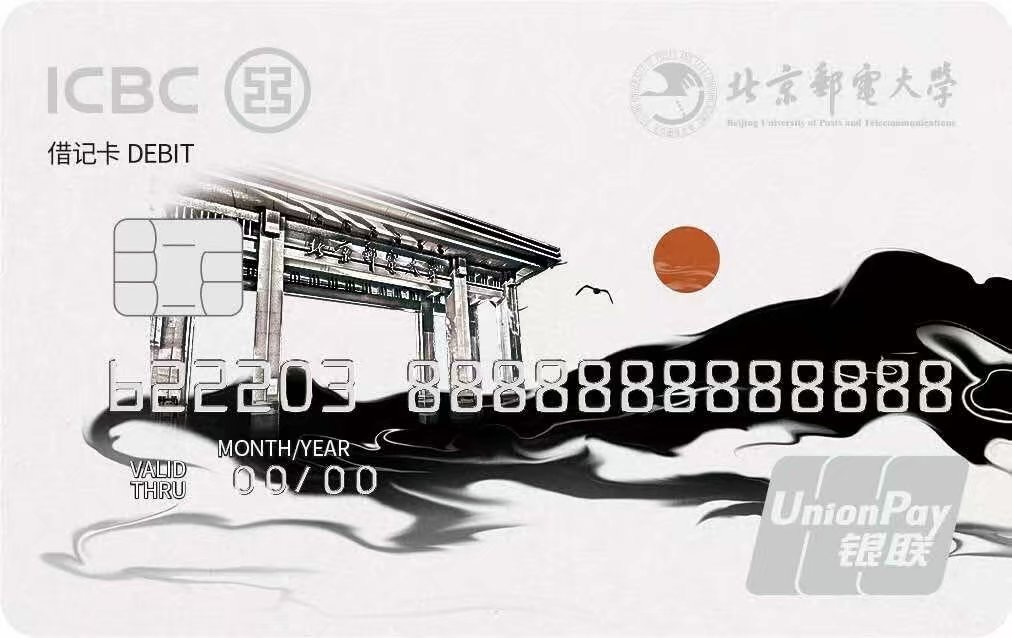
\includegraphics[width=0.55\textwidth]{images/card.jpg}
\end{center}

具体办理方法见录取通知书附带的新生指南。每人每月将获得北京市提供的60元生活补助(会发放到上述银行卡或校园一卡通中)。另有注册困难生的补助若干。

\faq{他们说的什么果园梨园树莓啊,都是什么东西啊?}

一些简称:
\begin{itemize}
    \item 果园:国际学院
    \item 梨园:理学院
    \item 树莓:数字媒体与艺术学院
    \item 青梅:北邮青年新媒体中心
\end{itemize}

课程简称:
\begin{itemize}
    \item 数电:数字系统基础
    \item 计组:计算机组织与结构(对于软件工程专业)
    \item 自动机:形式语言与自动机
    \item 大雾:基础物理学(对于软件工程专业)
    \item 软导:软件工程专业导论
    \item 思修,史纲,马原,毛概(也叫毛中特):四门\footnote{按教育部的要求,现在增加了《习近平中国特色社会主义概论》和“党史”“新中国史”“改革开放史”“社会主义发展史”四选一,共六门}思政课,按顺序一学期一门,分别为《思想道德基础与法律修养》、《中国近现代史纲要》、《马克思主义基本原理概论》、《毛泽东思想和中国特色社会主义理论体系概论》
\end{itemize}

\faq{我想参加某某竞赛/活动,如何报名/找到组织?}

对于以个人名义参加的竞赛或活动,一般来说等待学校发布相关通知后按要求报名即可。

对于需要组队参加的竞赛或活动,通常都需要一个指导老师并通过学校集体报名。程序设计竞赛由集训队负责组织,其他情况类似的竞赛一般也有现成的老师负责,你可以在各种群里询问学长学姐,相信很快就能找到组织。

如果你参加的比赛之前从未有人参加过,而又必须通过学校报名等等,你可以向学院和团委等有关部门询问相关事项。

\faq{暑假我应该预习一些课程吗?}

强烈建议暑假不要花时间在学习高等数学或者线性代数等诸如此类的事情上,预习这些课程最多只能你在开学后的初期获得薄弱优势,还会给你造成一些自我认知上的错觉。实际上如果不转变学习思维,这样的无效预习只会浪费掉你人生中(几乎唯一的)最没有压力的暑假。

如果你一定要在暑假学习某种知识,优先建议发展一门专业无关的兴趣爱好。实在没有的话,可以提前接触编程,在暑假过程中摸索“思维的转化”,可能很痛苦,但四处碰壁的过程中是更为扎实的“炼气期”,或许能为未来的修行积累经验。
